\documentclass[11pt]{article}

\usepackage[margin=1in]{geometry}
\usepackage{amsmath}
\usepackage{amssymb}
\usepackage[titles]{tocloft}
\usepackage{graphicx}

\usepackage{tikz}
\usetikzlibrary{arrows.meta,positioning}
\usepackage[hidelinks]{hyperref}

\title{SENA: Sparse-stock Estimation with Nonstationary Adaptation}
\author{Monysovann Ly}
\date{\today}

\setlength{\parindent}{0pt}
\setlength{\parskip}{1\baselineskip}

\begin{document}

\begin{titlepage}
\maketitle

\begin{abstract}
SENA (Sparse-stock Estimation with Nonstationary Adaptation) is a proposed Bayesian generative model for settings with a single business entity where services (and optionally retail SKUs) are sold but inventory is recorded intermittently. From sparse stock snapshots, SENA is designed to infer a plausible latent ledger of service demand, retail demand, order placements, receipts, and adjustments, while adapting to drift, seasonality, promotions, and occasional change points.

The model is designed to work with minimal inputs (inventory reports), but can optionally incorporate user-supplied time series and low-effort signals to improve identifiability.
Examples include prices, lead-time typical values and uncertainty ranges, optional order placed/received logs, ranked lists of top services/SKUs, service--SKU sharing masks, and stockout flags.

Its intended outputs are posterior inventory trajectories with uncertainty, demand-rate estimates and forecasts, stockout risk, and reorder policies (including safety stock and reorder points) under explicit service-level targets.
\end{abstract}

\vspace{1em}
\noindent\textbf{Keywords:} Bayesian inference; inventory reconstruction; stockout risk; demand drift; restocking policy; safety stock; reorder point.

\end{titlepage}

\tableofcontents
\newpage

\section{What SENA models}

\textbf{Scope.} SENA is designed for a single business entity with one internally coherent inventory process, where inventory is observed intermittently, direct sales logs may be missing, and operational decisions (stockout risk, reorder timing, safety stock) still require uncertainty-aware support.
No cross-business pooling is assumed.

\textbf{Contribution summary.}
\begin{enumerate}
  \item A proposed Bayesian state-space specification for a single business entity that reconstructs latent demand, order placements, receipts, and corrections from sparse stock snapshots.
  \item A practical identifiability strategy designed to absorb user-supplied optional signals (rankings, order placed/received logs, sharing masks, stockout flags, observed price series, and noisy lead-time inputs).
  \item A planning layer that maps posterior latent demand and latent lead-time dynamics into intended stockout-risk, days-of-cover, and reorder-policy outputs.
  \item A drift-aware design (gradual, seasonal, abrupt) intended to adapt to behavior change without pooling across different businesses.
\end{enumerate}

\textbf{Content.} The next sections define the proposed generative model, optional observation channels, prior defaults, and posterior outputs; later sections outline evaluation expectations and practical inference workflows needed before publication-ready empirical claims can be made.

\subsection*{High-level diagram}

\begin{center}
\resizebox{\textwidth}{!}{%
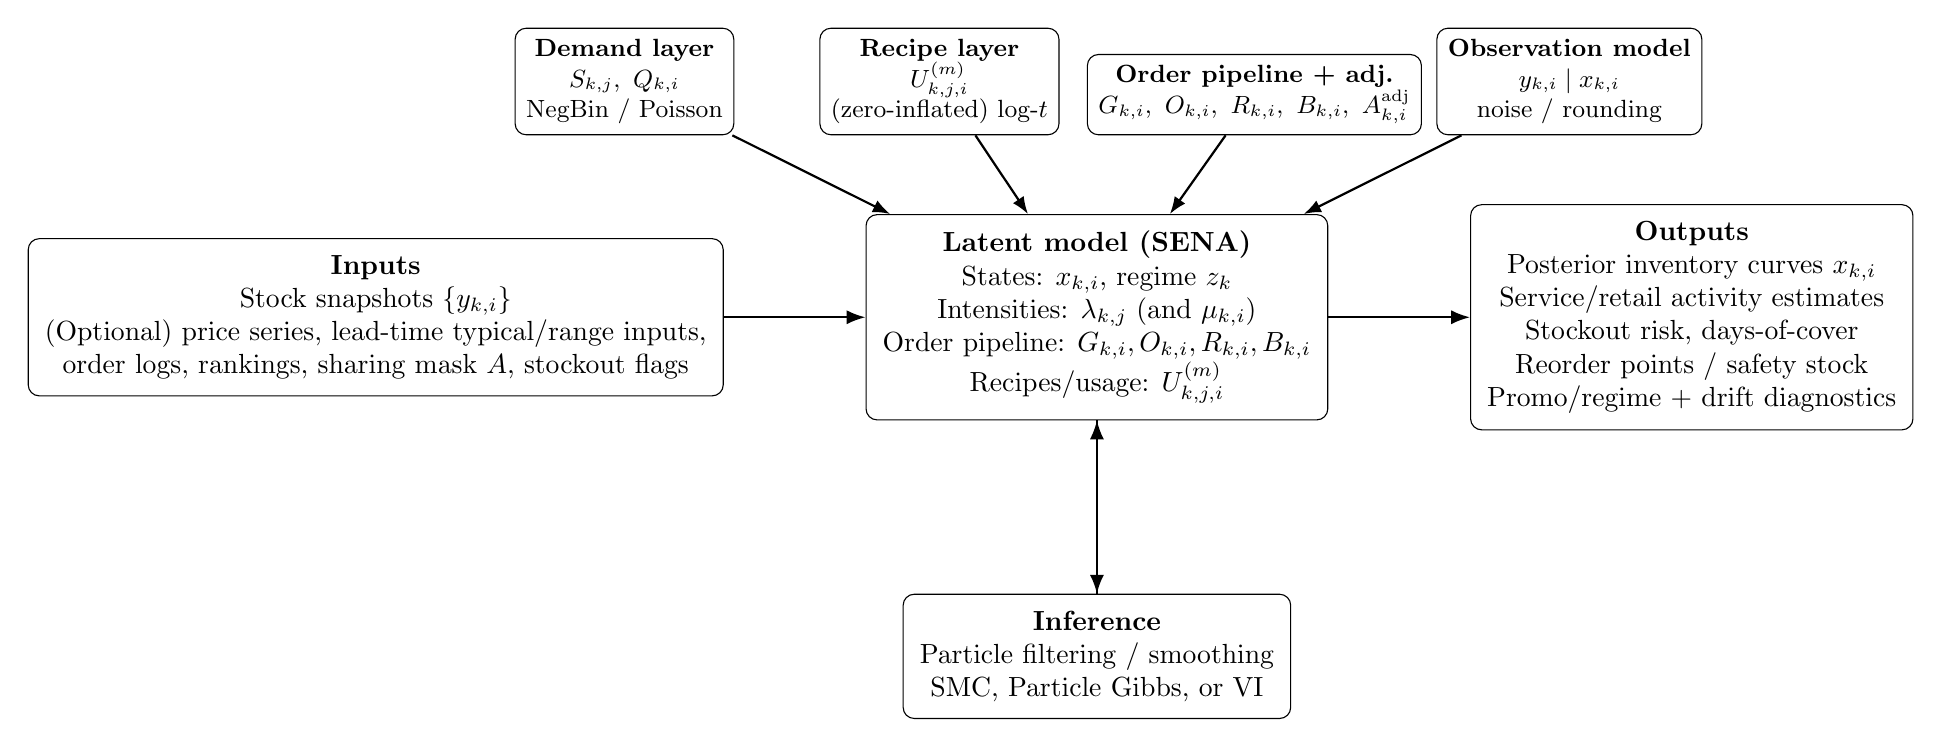
\begin{tikzpicture}[
  box/.style={draw, rounded corners, align=center, inner sep=6pt},
  subbox/.style={draw, rounded corners, align=center, inner sep=4pt, font=\small},
  arr/.style={-{Latex[length=2.4mm]}, thick},
  subarr/.style={-{Latex[length=2.2mm]}, thick}
]

\node[box] (inputs) {\textbf{Inputs}\\
Stock snapshots $\{y_{k,i}\}$\\
(Optional) price series, lead-time typical/range inputs,\\order logs, rankings, sharing mask $A$, stockout flags};

\node[box, right=18mm of inputs] (model) {\textbf{Latent model (SENA)}\\
States: $x_{k,i}$, regime $z_k$\\
Intensities: $\lambda_{k,j}$ (and $\mu_{k,i}$)\\
Order pipeline: $G_{k,i},O_{k,i},R_{k,i},B_{k,i}$\\
Recipes/usage: $U^{(m)}_{k,j,i}$};

\node[box, right=18mm of model] (outputs) {\textbf{Outputs}\\
Posterior inventory curves $x_{k,i}$\\
Service/retail activity estimates\\
Stockout risk, days-of-cover\\
Reorder points / safety stock\\
Promo/regime + drift diagnostics};

% Components that feed into SENA
\node[subbox, above=10mm of model, xshift=-60mm] (demand) {\textbf{Demand layer}\\
$S_{k,j},\ Q_{k,i}$\\
NegBin / Poisson};

\node[subbox, above=10mm of model, xshift=-20mm] (recipes) {\textbf{Recipe layer}\\
$U^{(m)}_{k,j,i}$\\
(zero-inflated) log-$t$};

\node[subbox, above=10mm of model, xshift=20mm] (restock) {\textbf{Order pipeline + adj.}\\
$G_{k,i},\ O_{k,i},\ R_{k,i},\ B_{k,i},\ A^{\mathrm{adj}}_{k,i}$};

\node[subbox, above=10mm of model, xshift=60mm] (obs) {\textbf{Observation model}\\
$y_{k,i}\mid x_{k,i}$\\
noise / rounding};

\node[box, below=22mm of model] (inference) {\textbf{Inference}\\Particle filtering / smoothing\\SMC, Particle Gibbs, or VI};

\draw[arr] (inputs) -- (model);
\draw[arr] (model) -- (outputs);

\draw[subarr] (demand) -- (model);
\draw[subarr] (recipes) -- (model);
\draw[subarr] (restock) -- (model);
\draw[subarr] (obs) -- (model);

\draw[arr] (model) -- (inference);
\draw[arr] (inference) -- (model);

\end{tikzpicture}%
}%
\end{center}

Time is indexed by report times $t_1 < \dots < t_K$.
Transition equations are evaluated on intervals $[t_{k-1},t_k]$ for $k=2,\dots,K$, with irregular gaps ($\Delta t_k = t_k - t_{k-1}$).
For irregular intervals, stochastic state increments are scaled by $\sqrt{\Delta t_k}$ and accumulation moments by $\Delta t_k$.

\textbf{Indices}
\begin{enumerate}
  \item SKU ($i \in \{1,\dots,I\}$)
  \item Service ($j \in \{1,\dots,J\}$)
  \item Bundle or promo service ($b \in \{1,\dots,N_{\mathrm{bundle}}\}$) (optional explicit bundle types)
\end{enumerate}

\textbf{Definitions and notation}
\begin{enumerate}
  \item Report times: $t_1 < \dots < t_K$.
  \item Transition intervals: $k\in\{2,\dots,K\}$ with $\Delta t_k = t_k - t_{k-1}$.
  \item Interval-indexed transition events $(D_{k,i},G_{k,i},O_{k,i},s_{k,i},R_{k,i},C_{k,i},A^{\mathrm{adj}}_{k,i})$ are defined for $k=2,\dots,K$ only; at $k=1$ only report-indexed states (e.g., $x_{1,i},B_{1,i}$) are defined.
  \item Initial states at the first report ($k=1$):
  \[
    x_{1,i}=x^{\mathrm{init}}_i,\qquad B_{1,i}=B^{\mathrm{init}}_i=0,\qquad x^{\mathrm{init}}_i\ge 0.
  \]
  This is an enforced model assumption: SENA does not represent latent pre-$t_1$ outstanding orders, and receipts are generated only from order batches placed in transition intervals $u=2,\dots,K$.
  Treat $x^{\mathrm{init}}_i$ as latent with a data-independent prior
  \[
    x^{\mathrm{init}}_i\sim \text{Normal}^+(m^{x0}_i,(s^{x0}_i)^2),\qquad m^{x0}_i\ge 0,\ s^{x0}_i>0.
  \]
  This keeps initialization independent of observed reports; $y_{1,i}$ enters only through the observation likelihood.
  \item Inventory state: $x_{k,i}$ is on-hand inventory of SKU $i$ immediately after report $k$.
  \item Reported stock: $y_{k,i}$ is a noisy/rounded observation of $x_{k,i}$.
  \item Inventory update in interval $k$ for SKU $i$ (for $k=2,\dots,K$):
  \begin{enumerate}
    \item Let $D_{k,i}\ge 0$ denote \emph{latent (unconstrained) demand/usage} in the interval.
    \item Let $G_{k,i}\in\{0,1\}$ indicate whether an order is placed in interval $k$, let $O_{k,i}\ge0$ be placed quantity, and let $s_{k,i}\in[t_{k-1},t_k]$ be the within-interval placement timestamp.
    \item Let $R_{k,i}\ge0$ be quantity \emph{received} during interval $k$ from previously placed orders.
    \item Let $B_{k,i}\ge0$ denote in-transit pipeline inventory right after interval $k$:
    \[
      B_{k,i}=\max\bigl\{0,\ B_{k-1,i}+O_{k,i}-R_{k,i}\bigr\}.
    \]
    \item Let $C_{k,i}$ denote \emph{realized} consumption/usage, capped by available inventory:
    \[
      C_{k,i} = \min\bigl\{D_{k,i},\ x_{k-1,i} + R_{k,i}\bigr\}.
    \]
    \item Let $A^{\mathrm{adj}}_{k,i}$ be a signed inventory correction (can be positive or negative).
    \item Define the pre-clamp inventory proposal
    \[
      x^\star_{k,i} = x_{k-1,i} + R_{k,i} - C_{k,i} + A^{\mathrm{adj}}_{k,i}.
    \]
    \item Then the inventory state update is
    \[
      x_{k,i} = \max\bigl\{0,\ x^\star_{k,i}\bigr\}.
    \]
  \end{enumerate}
  Here $R_{k,i}$ is generated by a lead-time-driven pipeline from historical order placements.

  \item Services and retail:
  \begin{enumerate}
    \item $S_{k,j}$: \emph{latent demand-side} count of service $j$ instances in interval $k$.
    \item $Q_{k,i}$: \emph{latent demand-side} retail quantity of SKU $i$ in interval $k$ (if modeled).
    \item Optional explicit realized-sales quantities: $S^{\mathrm{real}}_{k,j}$ and $Q^{\mathrm{real}}_{k,i}$, with
    \[
      0\le S^{\mathrm{real}}_{k,j}\le S_{k,j},\qquad 0\le Q^{\mathrm{real}}_{k,i}\le Q_{k,i}.
    \]
  \end{enumerate}
  \item Regimes: $z_k$ is a discrete regime label controlling dispersion and/or recipe shifts.
  \begin{enumerate}
    \item \textbf{Normal:} baseline behavior; demand and recipes follow their usual drift/seasonal dynamics.

    \item \textbf{Spike:} short-lived demand surge (e.g., an event day). Typically increases mean intensity (larger $\lambda_{k,j}$ and/or $\mu_{k,i}$) and may increase dispersion (smaller active-regime dispersion values $\kappa_{r,j}$ / $\phi_{r,i}$ with $r=z_k$).

    \item \textbf{Lull:} unusually quiet interval. Typically decreases intensities and may also reduce dispersion (closer to Poisson-like behavior).

    \item \textbf{Stockout-constrained:} latent demand exists, but realized sales/usage are capped when inventory hits (or approaches) zero. In this regime, demand-side quantities ($S_{k,j},Q_{k,i}$) can exceed realized quantities ($S^{\mathrm{real}}_{k,j},Q^{\mathrm{real}}_{k,i}$), and observed consumption is interpreted as \emph{censored} demand. The posterior favors trajectories with $\min_t x_i(t) \approx 0$ for at least one binding SKU.

    \item \textbf{Promo:} promotion period that shifts the service mix and/or usage recipes (e.g., different average inputs per service). Operationally this can mean shifted $\lambda_{k,j}$, different dispersions, and/or shifted recipe means $\mu^{\mathrm{use}}_{k,j,i}$.

    \item \textbf{Correction:} bookkeeping/measurement correction (late entry, recount, unit conversion, write-off). This regime increases the probability and/or scale of inventory corrections $A^{\mathrm{adj}}_{k,i}$ and can also inflate observation noise $\sigma_{\text{obs},i}$ for the affected interval.
  \end{enumerate}

  For notation clarity, let $r\in\{1,\dots,R\}$ index regime types and define regime-specific parameter tables
  $\kappa_{r,j},\ \phi_{r,i},\ m^{\mathrm{adj}}_{r,i},\ s^{\mathrm{adj}}_{r,i}$.
  In interval $k$, evaluate these parameters at $r=z_k$ inside likelihood and transition terms.

  \item Distribution notation: $\text{Normal}^+(m,s^2)$ denotes a Normal$(m,s^2)$ truncated to $\mathbb{R}_{\ge 0}$.
  \item LogNormal convention: throughout, $\text{LogNormal}(\mu,\sigma)$ means $(\log X)\sim\text{Normal}(\mu,\sigma^2)$, so the second argument is the \emph{log-standard-deviation}.
\end{enumerate}

\textbf{Latent states and events}
Report-indexed states use $k=1,\dots,K$; transition-event quantities use $k=2,\dots,K$.
\begin{enumerate}
  \item $x_{k,i}$: true on-hand inventory of SKU $i$ right after report $k$
  \item $B_{k,i}$: in-transit (ordered but not yet received) inventory for SKU $i$
  \item $z_k$: discrete regime (normal, spike, lull, stockout-constrained, promo, correction)
  \item $\lambda_{k,j}$: time-varying service intensity for service $j$
  \item $\mu_{k,i}$: time-varying retail intensity for SKU $i$ (optional)
  \item $G_{k,i},O_{k,i},s_{k,i},R_{k,i}$: placement event, placed quantity, placement timestamp, and received quantity (defined on transition intervals $k=2,\dots,K$)
  \item $m^L_{k,i}, v^L_{k,i}$: latent lead-time mean (days) and latent lead-time variance state (days$^2$)
  \item Order-policy states: dynamic baseline/slope coefficients $\alpha_{k,i}, \beta_{k,i}$ and static sensitivities $\gamma_i, \xi_i$
  \item Order-size parameters: target inventory position $T^{\mathrm{ord}}_i$ and log-size coefficients $\alpha^{O}_i, \beta^{O}_i$
  \item $\text{age}_{k,i}$: time-since-last-order state (days) used in the placement policy
\end{enumerate}

\subsection*{Observed (required)}
\begin{enumerate}
  \item $y_{k,i}$: reported stock (noisy, possibly rounded)
\end{enumerate}

\subsection*{Observed (optional add-ons)}
\begin{enumerate}
  \item User-supplied exogenous price and lead-time summaries:
  \begin{enumerate}
    \item $p^{\mathrm{svc}}_{k,j}$: price for service $j$ during interval $k$
    \item $p^{\mathrm{ret}}_{k,i}$: price for retail SKU $i$ during interval $k$
    \item $\tilde m^L_{k,i}$: user-provided typical lead time (days) for SKU $i$ near interval $k$ (noisy and possibly delayed)
    \item $[\tilde L^{\mathrm{lo}}_{k,i},\tilde L^{\mathrm{hi}}_{k,i}]$: user-provided plausible lead-time range (days)
    \item $\tilde c^L_{k,i}\in\{1,\dots,C\}$ (optional): user-selected relative-variability class derived from the range (e.g., very stable, moderate, volatile)
  \end{enumerate}

  \item Ranked lists per interval $k$ (no quantities):
  \begin{enumerate}
    \item $r^{\mathrm{svc}}_k$: ordering of top services in $\Delta t_k$
    \item $r^{\mathrm{ret}}_k$: ordering of top retail SKUs in $\Delta t_k$ (if retail is used)
  \end{enumerate}

  \item Optional order-event logs per update:
  \begin{enumerate}
    \item $\tilde g^{\mathrm{ord}}_{k,i} \in \{0,1\}$: user indicates whether an order was placed for SKU $i$ in $\Delta t_k$
    \item $\tilde h^{\mathrm{rcv}}_{k,i} \in \{0,1\}$: user indicates whether a receipt arrived for SKU $i$ in $\Delta t_k$
    \item Optional approximate quantities: $\tilde O_{k,i}$ (placed) and $\tilde R_{k,i}$ (received)
  \end{enumerate}

  \item Service--SKU sharing mask (sparse recipe support):
  \begin{enumerate}
    \item $A_{j,i} \in \{0,1\}$: whether service $j$ can consume SKU $i$ (enables the connection)
    \item $\rho_{k,j,i} \in (0,1)$: probability that a given instance of service $j$ actually uses SKU $i$ in interval $k$ (optional)
  \end{enumerate}

  \item Stockout flags:
  \begin{enumerate}
    \item $o^{\mathrm{svc}}_{k,j} \in \{0,1\}$: whether service $j$ was unavailable at any point in $\Delta t_k$
    \item $o^{\mathrm{ret}}_{k,i} \in \{0,1\}$: whether retail SKU $i$ was unavailable at any point in $\Delta t_k$
  \end{enumerate}
\end{enumerate}

\section{Inventory dynamics}

For each SKU $i$, with initial states $(x_{1,i},B_{1,i})$ and enforced zero initial pipeline $B_{1,i}=0$, the transition recursions below apply for $k=2,\dots,K$ unless otherwise stated.
\begin{enumerate}
  \item Let $D_{k,i}\ge 0$ denote latent (unconstrained) demand/usage in the interval.
  \item Let $G_{k,i}\in\{0,1\}$ denote whether an order is placed, with placed quantity $O_{k,i}\ge0$ and placement timestamp $s_{k,i}\in[t_{k-1},t_k]$.
  \item Let $R_{k,i}\ge0$ denote receipt quantity in interval $k$ generated by the lead-time-driven order pipeline.
  \item Update in-transit pipeline as
  \begin{equation}\label{eq:inv-pipeline}
    B_{k,i}=\max\bigl\{0,\ B_{k-1,i}+O_{k,i}-R_{k,i}\bigr\}.
  \end{equation}
  \item Let $C_{k,i}$ denote realized consumption/usage, capped by available inventory:
  \begin{equation}\label{eq:inv-consumption-cap}
    C_{k,i} = \min\bigl\{D_{k,i},\ x_{k-1,i} + R_{k,i}\bigr\}.
  \end{equation}
  \item Define the pre-clamp inventory proposal
  \begin{equation}\label{eq:inv-preclamp}
    x^\star_{k,i} = x_{k-1,i} + R_{k,i} - C_{k,i} + A^{\mathrm{adj}}_{k,i}.
  \end{equation}
  \item Inventory updates as
  \begin{equation}\label{eq:inv-clamp-update}
    x_{k,i} = \max\bigl\{0,\ x^\star_{k,i}\bigr\}.
  \end{equation}
\end{enumerate}
Equations~\eqref{eq:inv-pipeline}--\eqref{eq:inv-clamp-update} define the core inventory transition used throughout the manuscript.

We decompose latent demand into service and retail components:
\[
  D_{k,i} = D^{\mathrm{svc}}_{k,i} + D^{\mathrm{ret}}_{k,i}.
\]

Here $A^{\mathrm{adj}}_{k,i}$ is a signed correction term (e.g., recount, write-off, unit conversion).

\subsection{Services sold, latent counts}

Service counts are latent and regime dependent:
\[
  S_{k,j} \sim \text{NegBin}(\lambda_{k,j}\,\Delta t_k,\ \kappa_{r,j}),\qquad r=z_k.
\]

Negative Binomial is the default because it tolerates burstiness. Poisson is a special case.

\subsection{Stochastic recipes, real-valued usage}

Each service instance consumes a random amount of each SKU.
Use $U^{(m)}_{k,j,i}$ as the canonical per-instance usage variable for instance index $m=1,\dots,S_{k,j}$, and define the interval-level aggregate
\[
  \bar U_{k,j,i}=\sum_{m=1}^{S_{k,j}} U^{(m)}_{k,j,i}.
\]

For one service $j$ and SKU $i$, per instance:
\[
  U^{(m)}_{k,j,i} \sim F_{k,j,i}.
\]

A strong default for positive real usage is a heavy-tailed log-Student-$t$ recipe:
\[
  \log U^{(m)}_{k,j,i} \sim \text{Student-}t_{\nu}\bigl(\mu^{\mathrm{use}}_{k,j,i},\ \sigma^{\mathrm{use}}_{j,i}\bigr).
\]

\textbf{Optional: zero-inflated (spike-and-slab) recipes.}

Setting $A_{j,i}=1$ means service $j$ \emph{can} consume SKU $i$, but it does not imply that SKU $i$ is used in \emph{every} instance of the service.
To capture ``sometimes uses SKU $i$, sometimes does not,'' introduce a per-instance usage indicator.

For each service instance $m=1,\dots,S_{k,j}$:
\[
  Z^{(m)}_{k,j,i} \sim \text{Bernoulli}(\rho_{k,j,i}),\qquad Z^{(m)}_{k,j,i} \in \{0,1\}.
\]
Then define
\[
  U^{(m)}_{k,j,i} = Z^{(m)}_{k,j,i} \cdot \tilde U^{(m)}_{k,j,i},\qquad \tilde U^{(m)}_{k,j,i} > 0,
\]
with a positive recipe distribution for the slab, e.g.
\[
  \log \tilde U^{(m)}_{k,j,i} \sim \text{Student-}t_{\nu}\bigl(\mu^{\mathrm{use}}_{k,j,i},\ \sigma^{\mathrm{use}}_{j,i}\bigr).
\]
If $A_{j,i}=0$, enforce $Z^{(m)}_{k,j,i}=0$ and hence $U^{(m)}_{k,j,i}=0$.

Service-driven latent demand contribution of SKU $i$ over the interval:
\[
  D^{\mathrm{svc}}_{k,i} = \sum_{j=1}^{J} \bar U_{k,j,i} = \sum_{j=1}^{J}\sum_{m=1}^{S_{k,j}} U^{(m)}_{k,j,i}.
\]

\subsection{Retail sales of SKUs}

If the user also sells SKUs as products, model retail quantity:
\[
  Q_{k,i} \sim \text{NegBin}(\mu_{k,i}\,\Delta t_k,\ \phi_{r,i}),\qquad r=z_k.
\]

Retail-driven latent demand contribution:
\[
  D^{\mathrm{ret}}_{k,i} = Q_{k,i} \cdot u^{\mathrm{ret}}_i,
\]

where $u^{\mathrm{ret}}_i$ is units per retail sale, often 1 or a known pack fraction.

When explicit realized transactions are required, introduce $S^{\mathrm{real}}_{k,j}$ and $Q^{\mathrm{real}}_{k,i}$ as censoring-adjusted quantities with
\[
  0\le S^{\mathrm{real}}_{k,j}\le S_{k,j},\qquad 0\le Q^{\mathrm{real}}_{k,i}\le Q_{k,i}.
\]
If external prices are provided, define optional realized revenue from realized quantities only:
\[
  \text{Rev}^{\mathrm{real}}_k = \sum_j p^{\mathrm{svc}}_{k,j} S^{\mathrm{real}}_{k,j} + \sum_i p^{\mathrm{ret}}_{k,i} Q^{\mathrm{real}}_{k,i}.
\]
More generally, any financial KPI should use realized quantities (or realized consumption $C_{k,i}$), not latent demand-side quantities; the time-varying demand dynamics used for these quantities are defined in Section~\ref{sec:drift-handling}.

\subsection{Adjustments and shrinkage}

Model adjustments as signed inventory corrections:
\[
  A^{\mathrm{adj}}_{k,i} \sim \text{Normal}\bigl(m^{\mathrm{adj}}_{r,i}\,\Delta t_k,\ (s^{\mathrm{adj}}_{r,i})^2\,\Delta t_k\bigr),\qquad r=z_k.
\]

Interpretation:
\begin{enumerate}
  \item $A^{\mathrm{adj}}_{k,i}<0$ corresponds to shrinkage/write-offs (waste, spoilage, theft).
  \item $A^{\mathrm{adj}}_{k,i}>0$ corresponds to upward corrections (late entries, recounts, unit conversion fixes).
\end{enumerate}

Inventory is still clamped at zero via Eq.~\eqref{eq:inv-clamp-update}.

\subsection{Restocking as a policy with an explicit order pipeline}

SENA separates replenishment into \emph{order placement} and \emph{receipt arrival}. This is necessary when lead times are noisy and possibly drifting.
For all recursions in this subsection, $k=2,\dots,K$ unless otherwise stated.

\textbf{Order placement event and size.} Let $G_{k,i}\in\{0,1\}$ indicate whether SKU $i$ is ordered in interval $k$ ($k=2,\dots,K$):
\[
  G_{k,i} \sim \text{Bernoulli}(\pi^{\mathrm{ord}}_{k,i}).
\]
Use a logistic placement policy
\[
  \text{logit}(\pi^{\mathrm{ord}}_{k,i}) = \alpha_{k,i} + \beta_{k,i} x_{k-1,i} + \gamma_i\,\text{age}_{k-1,i} + \xi_i B_{k-1,i},\qquad k=2,\dots,K,
\]
where lower on-hand inventory usually increases order propensity and larger in-transit pipeline $B_{k-1,i}$ usually decreases it.

Use dynamic coefficients for baseline and stock sensitivity with random-walk transitions and shrinkage via small innovation scales:
\[
  \alpha_{1,i}\sim\text{Student-}t_3(0,2.5),\qquad \beta_{1,i}\sim\text{Student-}t_3(0,2.5),
\]
\[
  \alpha_{k,i}=\alpha_{k-1,i}+\sqrt{\Delta t_k}\,\epsilon^{\alpha}_{k,i},\qquad
  \beta_{k,i}=\beta_{k-1,i}+\sqrt{\Delta t_k}\,\epsilon^{\beta}_{k,i},\qquad k=2,\dots,K,
\]
\[
  \epsilon^{\alpha}_{k,i}\sim\text{Normal}(0,\sigma^2_{\alpha,i}),\qquad
  \epsilon^{\beta}_{k,i}\sim\text{Normal}(0,\sigma^2_{\beta,i}).
\]
Smaller $\sigma_{\alpha,i},\sigma_{\beta,i}$ imply stronger shrinkage toward a near-static policy; larger values allow faster policy adaptation.

Define the age state (in days) at report time $t_k$ as elapsed time since the most recent placement for SKU $i$:
\[
  \text{age}_{1,i}=a^{\text{init}}_i,\qquad a^{\text{init}}_i\ge 0,
\]
\[
  \text{age}_{k,i}=
  \begin{cases}
    0, & \text{if } G_{k,i}=1,\\
    \text{age}_{k-1,i}+\Delta t_k, & \text{if } G_{k,i}=0.
  \end{cases}\qquad k=2,\dots,K.
\]
Thus the placement policy for interval $k$ uses $\text{age}_{k-1,i}$, the start-of-interval age.
Default initialization uses $a^{\text{init}}_i=0$ when no historical placement timestamp is available; otherwise set $a^{\text{init}}_i$ to time since the last known order at $t_1$.

To make order size reproducible, define the start-of-interval inventory-position gap
\[
  g^{O}_{k,i}=\bigl(T^{\mathrm{ord}}_i-x_{k-1,i}-B_{k-1,i}\bigr)_+,\qquad T^{\mathrm{ord}}_i>0,\qquad k=2,\dots,K,
\]
where $T^{\mathrm{ord}}_i$ is a SKU-specific target inventory position.
Then define the LogNormal location parameter by
\[
  \mu^{O}_{k,i}=\alpha^{O}_i+\beta^{O}_i\,g^{O}_{k,i},\qquad \beta^{O}_i\ge 0,\qquad k=2,\dots,K.
\]
Thus, conditional on placing an order, larger shortfalls between the target inventory position and the current inventory position $x_{k-1,i}+B_{k-1,i}$ imply larger expected order sizes on the log scale.

Placed quantity is
\[
  O_{k,i} \sim
  \begin{cases}
    0 & \text{if } G_{k,i}=0,\\
    \text{LogNormal}(\mu^{O}_{k,i},\ \sigma^{O}_i) & \text{if } G_{k,i}=1.
  \end{cases}
\]

To avoid boundary-time ambiguity, define an explicit within-interval placement timestamp
\[
  s_{k,i}=t_{k-1}+\rho^{\mathrm{ord}}_{k,i}\,\Delta t_k,\qquad \rho^{\mathrm{ord}}_{k,i}\in[0,1],\qquad k=2,\dots,K.
\]
When exact placement times are unavailable, use a fixed convention for $\rho^{\mathrm{ord}}_{k,i}$ (default midpoint $0.5$; alternatives include start $0$ or end $1$). If finer event data are available, $\rho^{\mathrm{ord}}_{k,i}$ can be observed directly or treated as latent.

\textbf{Latent lead-time process.} For each SKU, introduce latent lead-time mean and variance states:
\[
  \ell_{k,i}=\log m^L_{k,i},\qquad \psi_{k,i}=\log v^L_{k,i}.
\]
Here $v^L_{k,i}$ denotes lead-time variance (days$^2$), not lead-time standard deviation.
Initialize these lead-time random-walk states at $k=1$ via
\[
  \ell_{1,i}\sim\text{Normal}(m_{L,i},s_{L,i}^2),\qquad
  \psi_{1,i}\sim\text{Normal}(m_{v,i},s_{v,i}^2).
\]
With irregular intervals, use random-walk dynamics with heavy tails and $\sqrt{\Delta t_k}$ scaling:
\[
  \ell_{k,i}=\ell_{k-1,i}+\sqrt{\Delta t_k}\,\epsilon^{\ell}_{k,i},\qquad
  \psi_{k,i}=\psi_{k-1,i}+\sqrt{\Delta t_k}\,\epsilon^{\psi}_{k,i},\qquad k=2,\dots,K,
\]
\[
  \epsilon^{\ell}_{k,i}\sim\text{Student-}t_{\nu_L}(0,\sigma_{L,i}),\qquad
  \epsilon^{\psi}_{k,i}\sim\text{Student-}t_{\nu_v}(0,\sigma_{v,i}),\qquad k=2,\dots,K.
\]

\textbf{Lead-time-driven receipts.} The default lead-time family is LogNormal, with lead time treated as a \emph{continuous} positive duration (days).
For each order batch placed in transition interval $u=2,\dots,K$ with quantity $O_{u,i}$, map mean/variance pair $(m^L_{u,i},v^L_{u,i})$ to LogNormal parameters via Eq.~\eqref{eq:leadtime-map}:
\begin{equation}\label{eq:leadtime-map}
  \sigma_{L,u,i}=\sqrt{\log\!\left(1+\frac{v^L_{u,i}}{(m^L_{u,i})^2}\right)},\qquad
  \mu_{L,u,i}=\log m^L_{u,i}-\tfrac{1}{2}\sigma^2_{L,u,i},
\end{equation}
and sample with Eq.~\eqref{eq:leadtime-draw}:
\begin{equation}\label{eq:leadtime-draw}
  L^{\mathrm{ord}}_{u,i} \sim \text{LogNormal}(\mu_{L,u,i},\sigma_{L,u,i}).
\end{equation}
Define arrival time
\[
  a_{u,i}=s_{u,i}+L^{\mathrm{ord}}_{u,i},\qquad u=2,\dots,K.
\]
Under this baseline specification, only post-$t_1$ order batches can generate receipts, so the initial in-transit pipeline is fixed at $B_{1,i}=0$ rather than modeled through latent pre-$t_1$ pseudo-orders.
Received quantity in interval $k$ is then assigned by Eq.~\eqref{eq:receipt-assignment}:
\begin{equation}\label{eq:receipt-assignment}
  R_{k,i}=\sum_{u=2}^{k} O_{u,i}\,\mathbf{1}\{t_{k-1}<a_{u,i}\le t_k\},\qquad k=2,\dots,K.
\end{equation}
This timestamp-based assignment is the default for irregular reports. If an integer-day convention is required, use
\[
  L^{\mathrm{ord,day}}_{u,i}=\max\{1,\mathrm{round}(L^{\mathrm{ord}}_{u,i})\}
\]
before forming $a_{u,i}$.

The in-transit pipeline transition is
\[
  B_{k,i}=\max\bigl\{0,\ B_{k-1,i}+O_{k,i}-R_{k,i}\bigr\}.
\]

Therefore, lead-time uncertainty enters the \emph{generative inventory transition} through $R_{k,i}$ and $B_{k,i}$, not only through downstream planning formulas.

\section{Promotions and bundles}

\textbf{Motivation.} Sparse inventory snapshots create an ill-posed inverse problem: many different latent demand paths can explain the same observed stock changes.
Promotions and bundles are two common real-world causes of structured, short-lived departures from baseline demand and usage.
Modeling them explicitly is hypothesized to reduce misattribution risk (e.g., incorrectly attributing promo-driven inventory drops to long-run drift) and to improve identifiability by introducing interpretable structure (regime shifts and multi-SKU bundle signatures) that better matches how businesses actually operate.
These claims are treated as falsifiable hypotheses and are tested under the evaluation protocol in Section~\ref{sec:eval-protocol}.

SENA supports two mechanisms; both can be used together.

\subsection{Promotions as regimes}

Regime $z_k$ changes service mix, prices, and recipe parameters.

In the \textbf{promo} regime, the model allows systematic departures from baseline behavior, for example:
\begin{enumerate}
  \item \textbf{Demand lift and mix shift:} services may become more (or less) frequent, so the service intensities $\lambda_{k,j}$ can shift relative to non-promo periods. Importantly, the \emph{composition} of demand across services can change, not just the total volume.

  \item \textbf{Recipe/usage shift:} promotions can change how SKUs are consumed per service (e.g., different bundle contents, portion sizes, substitutions, or free add-ons). This is captured by allowing recipe parameters---especially the recipe means $\mu^{\mathrm{use}}_{k,j,i}$ (and optionally dispersions $\sigma^{\mathrm{use}}_{j,i}$)---to shift under promo.

  \item \textbf{Dispersion changes:} promos can increase burstiness and heterogeneity across days, which can be modeled via regime-specific overdispersion (e.g., smaller $\kappa_{r,j}$ for service counts, and smaller $\phi_{r,i}$ for retail counts if retail is modeled, evaluated at $r=z_k$).

  \item \textbf{Price and bundle effects (with observed price series):} with user-supplied prices $p^{\mathrm{svc}}_{k,j}$ / $p^{\mathrm{ret}}_{k,i}$ and bundle indicators, promo periods can be tied to observed price moves and mix shifts, which can improve identifiability of whether inventory drops are driven by higher demand, changed recipes, or both.
\end{enumerate}

Operationally, the promo regime is a structured way to let a small number of intervals ``break the rules'' of smooth drift/seasonality while still pooling information across time.

\subsection{Promotion-bundles as explicit services}

A common failure mode with sparse inventory reports is \emph{non-identifiability}: many different combinations of services could explain the same net SKU drawdown.
Explicit bundles are intended to reduce this ambiguity and are evaluated under Section~\ref{sec:eval-protocol}.

Introduce a set of bundle (or promo) service types indexed by $b\in\{1,\dots,N_{\mathrm{bundle}}\}$.
Each bundle $b$ is treated as a service with its own latent count $S_{k,b}$, price $p^{\mathrm{svc}}_{k,b}$ (if prices are tracked), and recipe distribution over SKUs $F_{k,b,i}$:
\begin{enumerate}
  \item \textbf{Bundle counts:} infer $S_{k,b}$ in the same way as any service count (e.g., via a Negative Binomial intensity model). This lets the model explain bursts of joint multi-SKU consumption by attributing them to bundle sales.

  \item \textbf{Bundle recipes:} bundles often consume a \emph{structured set} of SKUs (e.g., ``cut + style + shampoo'' or ``service + take-home product''). These multi-SKU signatures make it easier to distinguish bundle-driven consumption from coincidental co-movement across independent services.

  \item \textbf{Identifiability gain:} when inventory drops across several SKUs occur together, the posterior can put mass on bundle events instead of forcing implausible correlated spikes across many base services.

  \item \textbf{Interpretability:} the inferred $S_{k,b}$ provides a direct estimate of promo uptake (with uncertainty), which is often more actionable than changes in individual $\lambda_{k,j}$ alone.
\end{enumerate}

In this formulation, explicit bundles are expected to improve identifiability and interpretability.
Section~\ref{sec:eval-protocol} specifies ablations to test this claim.

\section{Drift handling: gradual, seasonal, abrupt}\label{sec:drift-handling}

\textbf{Motivation.} Real businesses rarely have stationary demand or stationary ``recipes'' for SKU usage: staff behavior changes, product lines evolve, prices and competitors move, and there are seasonal patterns.
Without drift, SENA would systematically misattribute slow changes to noise and overfit stale history.
Drift dynamics provide controlled forgetting: they let the posterior adapt to new behavior while still borrowing strength from past observations.

SENA models three complementary types of drift:
\begin{enumerate}
  \item \textbf{Gradual drift:} smooth, persistent evolution in demand rates and/or recipes, modeled as time-varying latent states (e.g., random-walk dynamics on $\log \lambda_{k,j}$ and optionally on recipe means $\mu^{\mathrm{use}}_{k,j,i}$).
  \item \textbf{Seasonal drift:} predictable periodic patterns (day-of-week, month-of-year), modeled as additive covariates (e.g., $w_{j,\text{dow}}$ and $w_{j,\text{month}}$) with shrinkage so they only activate when supported by data.
  \item \textbf{Abrupt drift:} rare structural breaks (new menu, supplier change, policy change, accounting correction), modeled via change points $c_k$ that allow partial resets or jumps in intensities and/or recipe parameters.
\end{enumerate}
For all recursions in this section, $k=2,\dots,K$ unless otherwise stated.

\subsection{Gradual drift via time-varying intensities}

\textbf{What drifts.} The main quantities that evolve over time are service intensities $\lambda_{k,j}$ (expected service activity per unit time) and, optionally, recipe means $\mu^{\mathrm{use}}_{k,j,i}$ (typical log-usage of SKU $i$ per instance of service $j$).

\textbf{Initial latent-state priors (at $k=1$).} To complete the random-walk specifications, initialize:
\[
  \log \lambda_{1,j}\sim\text{Normal}(m_{\lambda,j},s_{\lambda,j}^2),\qquad
  \log \mu_{1,i}\sim\text{Normal}(m_{\mu,i},s_{\mu,i}^2)\ \text{(if retail is modeled)},
\]
\[
  \mu^{\mathrm{use}}_{1,j,i}\sim\text{Normal}(m_{\mathrm{use},j,i},s_{\mathrm{use},j,i}^2)\ \text{(if recipe-mean drift is modeled)}.
\]

\textbf{Why drift on the log scale.} Intensities must stay positive ($\lambda_{k,j}>0$), so we model a random walk on $\log \lambda_{k,j}$.
This turns multiplicative changes (e.g., ``demand is up 20\%'') into approximately additive increments.

Service intensities drift with observed price covariates and irregular-interval scaling:
\[
  \log \lambda_{k,j} = \log \lambda_{k-1,j} + \sqrt{\Delta t_k}\,\epsilon_{k,j} + \beta^{\mathrm{svc}}_j\,\tilde p^{\mathrm{svc}}_{k,j},\qquad k=2,\dots,K,
\]
\[
  \epsilon_{k,j} \sim \text{Student-}t_{\nu_{\lambda}}\bigl(0,\ \sigma_{\lambda,j}\bigr),\qquad k=2,\dots,K,
\]
\[
  \tilde p^{\mathrm{svc}}_{k,j} = \log p^{\mathrm{svc}}_{k,j} - \frac{1}{k}\sum_{r=1}^{k} \log p^{\mathrm{svc}}_{r,j},\qquad k=1,\dots,K.
\]
This running-mean centering is causal and uses only information available through interval $k$.

Definitions:
\begin{enumerate}
  \item $\epsilon_{k,j}$ is the unit-time latent shock to the log-intensity for service $j$ in interval $k$; the realized interval increment is $\sqrt{\Delta t_k}\,\epsilon_{k,j}$.
  \item $\nu_{\lambda}$ is the degrees-of-freedom controlling tail-heaviness; smaller values allow occasional larger jumps.
  \item $\sigma_{\lambda,j}>0$ is the unit-time drift scale for service $j$; larger values mean faster-changing demand.
  \item $\beta^{\mathrm{svc}}_j$ is own-price elasticity on the log-intensity scale (typically negative).
  \item $\tilde p^{\mathrm{svc}}_{k,j}$ is causally centered log-price (running mean through $k$) so elasticity is separated from baseline level.
\end{enumerate}

Retail intensities drift analogously if used:
\[
  \log \mu_{k,i} = \log \mu_{k-1,i} + \sqrt{\Delta t_k}\,\epsilon^{\mathrm{ret}}_{k,i} + \beta^{\mathrm{ret}}_i\,\tilde p^{\mathrm{ret}}_{k,i},\qquad k=2,\dots,K,
\]
\[
  \epsilon^{\mathrm{ret}}_{k,i} \sim \text{Student-}t_{\nu_{\lambda}}\bigl(0,\ \sigma_{\mathrm{ret},i}\bigr),\qquad k=2,\dots,K,
\]
\[
  \tilde p^{\mathrm{ret}}_{k,i} = \log p^{\mathrm{ret}}_{k,i} - \frac{1}{k}\sum_{r=1}^{k} \log p^{\mathrm{ret}}_{r,i},\qquad k=1,\dots,K.
\]

Recipe mean drift (optional):
\[
  \mu^{\mathrm{use}}_{k,j,i} = \mu^{\mathrm{use}}_{k-1,j,i} + \sqrt{\Delta t_k}\,\eta_{k,j,i},\qquad k=2,\dots,K,
\]
\[
  \eta_{k,j,i} \sim \text{Normal}(0,\ \sigma^2_{\mu,j,i}),\qquad k=2,\dots,K.
\]

Here $\eta_{k,j,i}$ is the unit-time recipe-mean shock and $\sigma_{\mu,j,i}>0$ controls how quickly usage norms change.

\subsection{Seasonality as covariates with shrinkage}

Seasonality captures repeatable patterns (e.g., weekends) that are not well represented by a random walk.
For each service $j$, add calendar effects to the log-intensity:
\[
  \log \lambda_{k,j} \mathrel{+}= w_{j,\text{dow}}(\text{day of week}) + w_{j,\text{month}}(\text{month}).
\]

Here $w_{j,\text{dow}}(d)$ is the day-of-week effect (a 7-vector per service) and $w_{j,\text{month}}(m)$ is the month-of-year effect (a 12-vector per service).

\textbf{What ``shrinkage priors'' means.} A \emph{prior} is a probability distribution placed on an unknown parameter before seeing the current user's data.
A \emph{shrinkage prior} is a prior centered at 0 with most of its mass near 0, so that in the absence of strong evidence the posterior prefers small seasonal effects (i.e., $w\approx 0$).
This prevents overfitting when the time series is short or sparse.

A simple shrinkage choice is, for each service $j$,
\[
  w_{j,\text{dow}}(d) \sim \text{Normal}(0,\ \sigma^2_{\text{dow},j}),\qquad
  w_{j,\text{month}}(m) \sim \text{Normal}(0,\ \sigma^2_{\text{month},j}),
\]
with small scales $\sigma_{\text{dow},j},\sigma_{\text{month},j}$ (see Section~\ref{sec:hyperparams} for a hierarchical default).

\textbf{How $w$ is estimated.} During inference, these priors combine with the likelihood implied by the observed stock reports (and any optional signals) to produce a posterior over $w$.
If the data repeatedly show higher inferred demand on (say) weekends for service $j$, the posterior for the corresponding components of $w_{j,\text{dow}}$ moves away from 0; otherwise it stays near 0.

\subsection{Abrupt drift via occasional change points}

Abrupt drift handles rare structural breaks (new menu, staff changes, supplier changes).
We introduce a shared transition-interval change-point indicator:
\[
  c_k \sim \text{Bernoulli}(p_c),\qquad k=2,\dots,K,
\]

where $p_c\in(0,1)$ is the per-interval change-point probability.
The same $c_k$ is shared across services and SKUs in interval $k$, while component-specific reset weights determine which latent states actually jump.

For service intensities, replace the gradual-drift update with the mixture transition
\begin{equation}\label{eq:cp-service}
  \log \lambda_{k,j}=
  \begin{cases}
    \log \lambda_{k-1,j} + \sqrt{\Delta t_k}\,\epsilon_{k,j} + \beta^{\mathrm{svc}}_j\,\tilde p^{\mathrm{svc}}_{k,j}, & c_k=0,\\
    (1-\omega^{\mathrm{cp}}_{\lambda,j})\bigl(\log \lambda_{k-1,j} + \beta^{\mathrm{svc}}_j\,\tilde p^{\mathrm{svc}}_{k,j}\bigr) + \omega^{\mathrm{cp}}_{\lambda,j} b^{\lambda}_j + \zeta^{\lambda}_{k,j}, & c_k=1,
  \end{cases}
\end{equation}
with
\[
  \zeta^{\lambda}_{k,j}\sim\text{Normal}(0,(\sigma^{\mathrm{cp}}_{\lambda,j})^2),\qquad \omega^{\mathrm{cp}}_{\lambda,j}\in[0,1].
\]
Here $b^{\lambda}_j$ is a component-specific post-change baseline, $\omega^{\mathrm{cp}}_{\lambda,j}=0$ disables jumps for service $j$, and $\omega^{\mathrm{cp}}_{\lambda,j}=1$ gives a full reset to the new baseline up to change-point noise.

If retail intensity drift is enabled, use the analogous change-point transition
\begin{equation}\label{eq:cp-retail}
  \log \mu_{k,i}=
  \begin{cases}
    \log \mu_{k-1,i} + \sqrt{\Delta t_k}\,\epsilon^{\mathrm{ret}}_{k,i} + \beta^{\mathrm{ret}}_i\,\tilde p^{\mathrm{ret}}_{k,i}, & c_k=0,\\
    (1-\omega^{\mathrm{cp}}_{\mu,i})\bigl(\log \mu_{k-1,i} + \beta^{\mathrm{ret}}_i\,\tilde p^{\mathrm{ret}}_{k,i}\bigr) + \omega^{\mathrm{cp}}_{\mu,i} b^{\mu}_i + \zeta^{\mu}_{k,i}, & c_k=1,
  \end{cases}
\end{equation}
with
\[
  \zeta^{\mu}_{k,i}\sim\text{Normal}(0,(\sigma^{\mathrm{cp}}_{\mu,i})^2),\qquad \omega^{\mathrm{cp}}_{\mu,i}\in[0,1].
\]

If recipe-mean drift is enabled, use
\begin{equation}\label{eq:cp-recipe}
  \mu^{\mathrm{use}}_{k,j,i}=
  \begin{cases}
    \mu^{\mathrm{use}}_{k-1,j,i}+\sqrt{\Delta t_k}\,\eta_{k,j,i}, & c_k=0,\\
    (1-\omega^{\mathrm{cp}}_{\mathrm{use},j,i})\mu^{\mathrm{use}}_{k-1,j,i} + \omega^{\mathrm{cp}}_{\mathrm{use},j,i} b^{\mathrm{use}}_{j,i} + \zeta^{\mathrm{use}}_{k,j,i}, & c_k=1,
  \end{cases}
\end{equation}
with
\[
  \zeta^{\mathrm{use}}_{k,j,i}\sim\text{Normal}(0,(\sigma^{\mathrm{cp}}_{\mathrm{use},j,i})^2),\qquad \omega^{\mathrm{cp}}_{\mathrm{use},j,i}\in[0,1].
\]

Seasonal covariates continue to enter through the same additive terms after these state updates, so change points capture structural level shifts rather than recurring calendar effects.
If a block should not jump, fix its corresponding reset weights $\omega^{\mathrm{cp}}$ to $0$.

\section{Observation model for sparse stock reports}

Inventory is only observed intermittently, and reported values may be rounded or measured with error.
We model the reported stock as a noisy observation of the latent true on-hand inventory.

\textbf{Variables.}
\begin{enumerate}
  \item $x_{k,i}$ is the latent on-hand inventory of SKU $i$ immediately after report $k$.
  \item $y_{k,i}$ is the reported/measured stock value for SKU $i$ at report $k$.
  \item $\sigma_{\text{obs},i}>0$ is an SKU-specific observation-noise scale capturing counting error, scale/rounding noise, and minor reporting inconsistencies.
\end{enumerate}

\textbf{Gaussian observation model.} A simple default is:
\[
  y_{k,i} \sim \text{Normal}(x_{k,i},\ \sigma^2_{\text{obs},i}).
\]

\textbf{Rounding (optional).} If users tend to report in coarse increments (e.g., ``about 10''), treat $y_{k,i}$ as a rounded version of an underlying noisy measurement, e.g., by adding an explicit rounding operator or a mixture model that puts extra mass on common multiples.

\subsubsection*{Optional minimal user inputs as extra observations}

These inputs are designed to be low-effort (binary/categorical/ordinal) while materially improving identifiability.

\textbf{(i) Ranked lists of services / SKUs}

Users often know \emph{which} services/SKUs were most common in an interval, even if they do not know the exact counts.
SENA can incorporate this information as an \emph{ordinal} observation that constrains latent intensities.

\textbf{What the user provides.}
\begin{enumerate}
  \item $r^{\mathrm{svc}}_k$ is an ordering of the top services during interval $k$ (e.g., $[j_1 \succ j_2 \succ j_3]$).
  \item Optionally, $r^{\mathrm{ret}}_k$ is an ordering of the top retail SKUs during interval $k$.
\end{enumerate}

\textbf{What it means in the model.} If service $a$ is ranked above $b$ (denoted $a\succ b$), we interpret it as evidence that the activity rate for $a$ exceeded that of $b$ during interval $k$.
A simple (pairwise) likelihood is:
\[
  P(a \succ b \mid \lambda_{k,*}) = \sigma\!\left(\frac{\log \lambda_{k,a} - \log \lambda_{k,b}}{\tau}\right),
\]

where $\sigma(u)=1/(1+e^{-u})$ is the logistic function and $\tau>0$ is a \emph{temperature} controlling ranking noise.
As $\tau\to 0$, the ranking becomes nearly deterministic; larger $\tau$ makes rankings less informative.

\textbf{How a top-$N$ list becomes constraints.} If the list is $[j_1 \succ j_2 \succ \dots \succ j_N]$, add pairwise comparisons for all adjacent pairs $j_1\succ j_2$, $j_2\succ j_3$, \dots, $j_{N-1}\succ j_N$ (or, more strongly, for all pairs $j_a\succ j_b$ with $a<b$).
Items not listed are treated as ``unranked'' (no constraint) unless the user explicitly asserts they were below the top-$N$.

\textbf{Notes.} If ties are common, treat them as weak constraints (e.g., skip tied pairs or use a wide-$\tau$ likelihood).
More structured ranking likelihoods (e.g., Plackett--Luce) can be substituted, but the pairwise form is a robust default.

\textbf{(ii) Optional order placed/received logs}

With an explicit pipeline, two operational events matter: \emph{order placed} and \emph{order received}.
Optional user logs of either event help identify the replenishment path.

\textbf{What the user provides.}
\begin{enumerate}
  \item $\tilde g^{\mathrm{ord}}_{k,i}\in\{0,1\}$: whether an order was placed for SKU $i$ in $\Delta t_k$.
  \item $\tilde h^{\mathrm{rcv}}_{k,i}\in\{0,1\}$: whether any receipt arrived for SKU $i$ in $\Delta t_k$.
  \item Optional approximate quantities $\tilde O_{k,i}$ and $\tilde R_{k,i}$.
\end{enumerate}

\textbf{How it enters the model.}
\begin{enumerate}
  \item Treat $\tilde g^{\mathrm{ord}}_{k,i}$ as noisy observation of latent placement event $G_{k,i}$.
  \item Define $H^{\mathrm{rcv}}_{k,i}=\mathbf{1}\{R_{k,i}>0\}$ and treat $\tilde h^{\mathrm{rcv}}_{k,i}$ as noisy observation of $H^{\mathrm{rcv}}_{k,i}$.
  \item If quantity logs are supplied, use noisy measurement models centered on latent $O_{k,i}$ and $R_{k,i}$.
\end{enumerate}

These optional logs preserve low user burden while strongly constraining placement and arrival timing.

\textbf{(iii) Service--SKU sharing mask}

Another major source of non-identifiability is unknown recipe support: without constraints, any service can (in principle) consume any SKU.
A sparse support mask makes the inference more realistic and stable.

\textbf{What the user provides.} $A_{j,i}\in\{0,1\}$ indicates whether service $j$ can consume SKU $i$ at all (e.g., shampoo is used by ``wash'' services, but not by ``consultation'').
In practice this can come from a point-of-sale menu, a bill-of-materials template, or a simple checkbox UI.

\textbf{How it enters the model.} For canonical per-instance usage $U^{(m)}_{k,j,i}$:
\begin{enumerate}
  \item If $A_{j,i}=0$, enforce $U^{(m)}_{k,j,i}=0$ for all $k,m$ (structural zero).
  \item If $A_{j,i}=1$, draw each $U^{(m)}_{k,j,i}$ from the recipe distribution $F_{k,j,i}$ (or its spike-and-slab version).
\end{enumerate}

This focuses posterior mass on plausible explanations and reduces spurious cross-SKU attribution.

\textbf{(iv) Stockout flags}

Stockouts turn observed sales into \emph{censored} demand: low observed consumption may reflect lack of inventory, not lack of customers.
Stockout flags help the model distinguish these cases.

\textbf{What the user provides.}
\begin{enumerate}
  \item $o^{\mathrm{svc}}_{k,j}\in\{0,1\}$ indicates whether service $j$ was unavailable at any point during $\Delta t_k$.
  \item $o^{\mathrm{ret}}_{k,i}\in\{0,1\}$ indicates whether retail SKU $i$ was unavailable at any point during $\Delta t_k$.
\end{enumerate}

\textbf{How it enters the model.}
\begin{enumerate}
  \item If $o^{\mathrm{svc}}_{k,j}=1$, upweight trajectories where at least one required SKU (with $A_{j,i}=1$) hits (or closely approaches) zero during $\Delta t_k$, implying demand was partially blocked.
  \item If $o^{\mathrm{svc}}_{k,j}=0$, downweight trajectories that would force service $j$ to be stockout-constrained.

  \item If $o^{\mathrm{ret}}_{k,i}=1$, upweight trajectories where SKU $i$ hits (or closely approaches) zero during $\Delta t_k$.
  \item If $o^{\mathrm{ret}}_{k,i}=0$, downweight trajectories that would require SKU $i$ to be at (or near) zero for extended periods.
\end{enumerate}

\textbf{Default within-interval approximation.}
For stockout flags and stockout-risk summaries only, let $x_i(t)$ denote the auxiliary within-interval inventory path on $t\in[t_{k-1},t_k]$, defined by
\begin{equation}\label{eq:stockout-path}
  x_i(t)=
  \begin{cases}
    \max\!\left\{0,\ x_{k-1,i}+\sum_{u=2}^{k} O_{u,i}\,\mathbf{1}\{t_{k-1}<a_{u,i}\le t\}-\dfrac{t-t_{k-1}}{\Delta t_k}D_{k,i}\right\}, & t\in[t_{k-1},t_k),\\
    \max\!\left\{0,\ x_i(t_k^-)+A^{\mathrm{adj}}_{k,i}\right\}, & t=t_k.
  \end{cases}
\end{equation}
Thus latent demand is spread uniformly through the interval at rate $D_{k,i}/\Delta t_k$, receipts arrive as upward jumps at their explicit timestamps $a_{u,i}$, and the signed correction $A^{\mathrm{adj}}_{k,i}$ is applied as a single bookkeeping jump at report time $t_k$.
All statements in the bullets above about a SKU ``hitting zero during $\Delta t_k$'' are evaluated using Eq.~\eqref{eq:stockout-path}; the report-indexed transition recursion in Eqs.~\eqref{eq:inv-pipeline}--\eqref{eq:inv-clamp-update} remains unchanged.

In effect, the flags provide a qualitative observation about within-interval availability that is otherwise unidentifiable from sparse snapshot data.

\textbf{(v) Price and lead-time observations (noisy and delayed)}

Prices remain observed exogenous covariates. Lead time is instead modeled as latent, with user entries treated as noisy (and potentially stale) observations.

\textbf{What the user provides.}
\begin{enumerate}
  \item Service and retail price series: $p^{\mathrm{svc}}_{k,j}$ and $p^{\mathrm{ret}}_{k,i}$.
  \item Typical lead-time entry $\tilde m^L_{k,i}$ (days).
  \item A simple uncertainty proxy via range $[\tilde L^{\mathrm{lo}}_{k,i},\tilde L^{\mathrm{hi}}_{k,i}]$.
\end{enumerate}

\textbf{Range to ordinal variability map.}

Define a relative range width
\[
  w_{k,i}=\frac{\tilde L^{\mathrm{hi}}_{k,i}-\tilde L^{\mathrm{lo}}_{k,i}}{\max\!\left\{\frac{\tilde L^{\mathrm{hi}}_{k,i}+\tilde L^{\mathrm{lo}}_{k,i}}{2},\ \epsilon_L\right\}}.
\]
Here, $\epsilon_L>0$ denotes a fixed lead-time floor in day units, with default value $\epsilon_L=0.5$ day.
Map $w_{k,i}$ to an ordinal class $\tilde c^L_{k,i}\in\{1,\dots,C\}$ using thresholds $\rho_1<\dots<\rho_{C-1}$.

\textbf{Observation model for latent lead-time states.}

Let latent states be $\ell_{k,i}=\log m^L_{k,i}$ and $\psi_{k,i}=\log v^L_{k,i}$, where $v^L_{k,i}$ is lead-time variance (days$^2$).
Define the induced scale-free LogNormal shape parameter
\[
  \sigma_{L,k,i}=\sqrt{\log\!\left(1+\frac{v^L_{k,i}}{(m^L_{k,i})^2}\right)}.
\]
This quantity depends on relative rather than absolute lead-time spread, so it matches the scale-free range summary $w_{k,i}$.
Allow delayed updates via lag variables $\delta^{m}_{k,i},\delta^{c}_{k,i}\in\{0,1,\dots,D\}$.
Use clamped lag indices to avoid out-of-range references in early intervals:
\[
  k^{m,\star}_{k,i}=\max\{1,\ k-\delta^{m}_{k,i}\},\qquad
  k^{c,\star}_{k,i}=\max\{1,\ k-\delta^{c}_{k,i}\}.
\]

Typical lead-time entry:
\[
  \log \tilde m^L_{k,i} \sim \text{Normal}(\ell_{k^{m,\star}_{k,i},i},\ \tau_m^2).
\]
Ordinal uncertainty entry:
\[
  \tilde c^L_{k,i}\sim\text{OrderedLogit}\!\bigl(a_{0,i}+a_{1,i}\sigma_{L,k^{c,\star}_{k,i},i},\ \kappa_{1:C-1}\bigr),\quad a_{1,i}>0.
\]
Equivalently, one could use the exact LogNormal-compatible predictor
\[
  \log\!\left(1+\frac{v^L_{k^{c,\star}_{k,i},i}}{(m^L_{k^{c,\star}_{k,i},i})^2}\right)=\sigma^2_{L,k^{c,\star}_{k,i},i},
\]
which is a monotone reparameterization of the same scale-free latent variability.

Thus, users do not need to provide variance directly; range entries become an interpretable ordinal signal for latent relative lead-time variability rather than raw lead-time variance.

\subsubsection*{Hyperparameters and default priors}\label{sec:hyperparams}

This section lists suggested weakly-informative default priors for key hyperparameters.
Where possible, predictors should be scaled so that typical values are $O(1)$.

\textbf{Negative Binomial parameterization}

Assume $\text{NegBin}(m,\kappa)$ is parameterized by mean $m>0$ and dispersion $\kappa>0$:
\[
  E[Y]=m,\qquad \mathrm{Var}(Y)=m + \frac{m^2}{\kappa}.
\]
Then larger $\kappa$ is closer to Poisson.
(Equivalently, if you use a $(r,p)$ parameterization with $Y\sim\text{NegBin}(r,p)$ and support $Y\in\{0,1,2,\dots\}$, set
$r=\kappa$ and $p=\kappa/(\kappa+m)$ so that $E[Y]=m$.)

\textbf{Count dispersion}
\begin{enumerate}
  \item Service overdispersion table: $\kappa_{r,j} > 0$ for each regime $r$.
  \item Retail overdispersion table: $\phi_{r,i} > 0$ for each regime $r$.
\end{enumerate}
Default: initialize each regime table at $1$ (moderate overdispersion).
Use $\kappa_{r,j}=1$ and $\phi_{r,i}=1$ as starting values for inference/optimization.
Priors: $\kappa_{r,j} \sim \text{Exponential}(1)$ and $\phi_{r,i} \sim \text{Exponential}(1)$.

\textbf{Recipe noise and drift scales}
\begin{enumerate}
  \item Recipe log-scale noise: $\sigma^{\mathrm{use}}_{j,i} > 0$.
  \item Intensity drift scale: $\sigma_{\lambda,j} > 0$.
  \item Retail-intensity drift scale (if retail is modeled): $\sigma_{\mathrm{ret},i} > 0$.
  \item Recipe mean drift scale: $\sigma_{\mu,j,i} > 0$.
\end{enumerate}
The irregular-interval update is
\[
  \mu^{\mathrm{use}}_{k,j,i}=\mu^{\mathrm{use}}_{k-1,j,i}+\sqrt{\Delta t_k}\,\eta_{k,j,i},
  \qquad \eta_{k,j,i}\sim\text{Normal}(0,\sigma^2_{\mu,j,i}).
\]
Defaults: initialize $\sigma^{\mathrm{use}}_{j,i}$, $\sigma_{\lambda,j}$, $\sigma_{\mathrm{ret},i}$, and $\sigma_{\mu,j,i}$ at small values after standardizing units (e.g., $0.1$--$0.5$ on a log scale).
(Here $\sigma^{\mathrm{use}}_{j,i}$ appears in $\log U^{(m)}_{k,j,i}$, $\sigma_{\lambda,j}$ appears in the unit-time drift shock $\epsilon_{k,j}$ for $\log\lambda_{k,j}$, $\sigma_{\mathrm{ret},i}$ appears in $\epsilon^{\mathrm{ret}}_{k,i}$ for $\log\mu_{k,i}$, and $\sigma_{\mu,j,i}$ appears in the unit-time recipe drift shock $\eta_{k,j,i}$.)
Priors (weakly-informative):
\[
  \sigma^{\mathrm{use}}_{j,i},\ \sigma_{\lambda,j},\ \sigma_{\mathrm{ret},i},\ \sigma_{\mu,j,i} \sim \text{Half-}t_{4}(0,\ s),
\]
with a global scale $s>0$.
Default: set $s=1$ after scaling so that typical log-variations are $O(1)$.

\textbf{Zero-inflation probability (optional)}

If using the spike-and-slab recipe layer, $\rho_{k,j,i} \in (0,1)$ controls how often SKU $i$ is used when $A_{j,i}=1$.
A simple default is a weak prior:
\[
  \rho_{k,j,i} \sim \text{Beta}(1,1).
\]
Optionally, $\text{logit}(\rho_{k,j,i})$ can be given a drift model analogous to $\log \lambda_{k,j}$.

\textbf{Seasonality shrinkage (hierarchical).}
\[
  w_{j,\text{dow}}(d) \sim \text{Normal}(0,\ \sigma^2_{\text{dow},j}),\qquad
  w_{j,\text{month}}(m) \sim \text{Normal}(0,\ \sigma^2_{\text{month},j}).
\]
\[
  \sigma_{\text{dow},j} \sim \text{HalfNormal}(0,\ \tau_{\text{dow}}),\qquad
  \sigma_{\text{month},j} \sim \text{HalfNormal}(0,\ \tau_{\text{month}}).
\]
\[
  \tau_{\text{dow}} \sim \text{HalfNormal}(0,\ 1),\qquad
  \tau_{\text{month}} \sim \text{HalfNormal}(0,\ 1).
\]
Defaults: initialize $\tau_{\text{dow}}=0.3$ and $\tau_{\text{month}}=0.3$.
(Here $\tau_{\text{dow}}$ and $\tau_{\text{month}}$ are global hyperparameters controlling the typical magnitude of day-of-week and month effects across services; smaller values imply stronger shrinkage toward $w\approx 0$.)

\textbf{Observation noise}

Observation noise per SKU: $\sigma_{\text{obs},i} > 0$.
This parameter appears in the observation model
$y_{k,i}\sim\text{Normal}(x_{k,i},\sigma^2_{\text{obs},i})$ and summarizes counting error plus any effective noise induced by rounding.

Default: initialize $\sigma_{\text{obs},i}$ to the typical reporting resolution for SKU $i$ (e.g., if counts are usually within $\pm 1$, start at $1$; if reports are in steps of 5, start at $2$--$5$).
Prior: $\sigma_{\text{obs},i} \sim \text{HalfNormal}(0,\ s_{\text{obs}})$.
Default: set $s_{\text{obs}}=5$ in raw ``units'' (or $s_{\text{obs}}=1$ after scaling each SKU to unit variance).

\textbf{Adjustment model}

Recall the signed inventory-correction component
$A^{\mathrm{adj}}_{k,i} \sim \text{Normal}\bigl(m^{\mathrm{adj}}_{r,i}\,\Delta t_k,(s^{\mathrm{adj}}_{r,i})^2\,\Delta t_k\bigr)$ with $r=z_k$.
Here $s^{\mathrm{adj}}_{r,i}>0$ is the unit-time diffusion scale for corrections; over interval $\Delta t_k$, the correction standard deviation is $s^{\mathrm{adj}}_{r,i}\sqrt{\Delta t_k}$.

Default: initialize $s^{\mathrm{adj}}_{r,i}=1$ after scaling (or to a small number of physical units if unscaled).
Prior: $s^{\mathrm{adj}}_{r,i} \sim \text{Half-}t_{4}(0,\ s_{\text{adj}})$.
Default: set $s_{\text{adj}}=1$ after scaling.

\textbf{Order-policy coefficients}

These coefficients appear in the placement-propensity model
$\text{logit}(\pi^{\mathrm{ord}}_{k,i}) = \alpha_{k,i} + \beta_{k,i}x_{k-1,i} + \gamma_i\,\text{age}_{k-1,i} + \xi_i B_{k-1,i}$ for $k=2,\dots,K$.
For scaled predictors, use robust priors on the initial states and static sensitivities:
\[
  \alpha_{1,i},\ \beta_{1,i},\ \gamma_i,\ \xi_i \sim \text{Student-}t_{3}(0,\ 2.5).
\]
For dynamic drift scales, use shrinkage priors:
\[
  \sigma_{\alpha,i},\ \sigma_{\beta,i} \sim \text{Half-}t_4(0,\ s_{\text{ord}}).
\]
Default: set $s_{\text{ord}}=0.25$ after predictor scaling so order-policy coefficients evolve smoothly unless data support faster drift.

Interpretation: $\alpha_{k,i}$ is a time-varying baseline log-odds; $\beta_{k,i}$ is a time-varying stock-sensitivity term (often negative); $\gamma_i$ controls sensitivity to time since last order (log-odds change per day of age); $\xi_i$ controls sensitivity to in-transit pipeline inventory (often negative); $\sigma_{\alpha,i},\sigma_{\beta,i}$ govern how quickly order-policy behavior can drift.

\textbf{Order size model}

The LogNormal location is defined through a pipeline-aware inventory-position gap:
\[
  g^{O}_{k,i}=\bigl(T^{\mathrm{ord}}_i-x_{k-1,i}-B_{k-1,i}\bigr)_+,
  \qquad
  \mu^{O}_{k,i}=\alpha^{O}_i+\beta^{O}_i\,g^{O}_{k,i},
\]
with $T^{\mathrm{ord}}_i>0$ and $\beta^{O}_i\ge 0$.
Here $T^{\mathrm{ord}}_i$ is a SKU-specific target inventory position, $\alpha^{O}_i$ is a baseline log-order-size intercept, and $\beta^{O}_i$ controls how strongly order size increases when inventory position falls below target.
For scaled inventory-position inputs, use weakly informative priors
\[
  \alpha^{O}_i \sim \text{Student-}t_3(0,2.5),\qquad
  \beta^{O}_i \sim \text{Half-}t_4(0,\ s_{\beta O}),\qquad
  \log T^{\mathrm{ord}}_i \sim \text{Normal}(0,\ s_T^2).
\]
Defaults after scaling: initialize $\alpha^{O}_i=0$, $\beta^{O}_i=1$, and $T^{\mathrm{ord}}_i=1$, with $s_{\beta O}=1$ and $s_T=1$.

Order size noise: $\sigma^{O}_i > 0$.
This parameter appears in the LogNormal order-size model
$O_{k,i}\mid(G_{k,i}=1)\sim\text{LogNormal}(\mu^{O}_{k,i},\sigma^{O}_i)$ and controls multiplicative variability around the gap-based mean order size.

Default: initialize $\sigma^{O}_i=0.3$ (on the log scale) after scaling; smaller values imply more consistent order sizes for a given inventory-position gap.
Prior: $\sigma^{O}_i \sim \text{Half-}t_{4}(0,\ s_O)$.
Default: set $s_O=1$ after scaling.

\textbf{Change-point probability}

$p_c \in (0,1)$ is the per-interval change-point probability in
$c_k\sim\text{Bernoulli}(p_c)$ for transition intervals $k=2,\dots,K$.

Default: small (e.g. $0.01$ per interval), corresponding to an expected change-point spacing of about $1/p_c=100$ intervals.
Prior: $p_c \sim \text{Beta}(1,1)$.

\textbf{Change-point reset parameters}

When abrupt drift is enabled, each potentially jumping block has a reset weight $\omega^{\mathrm{cp}}\in[0,1]$, a post-change baseline $b$, and a change-point noise scale $\sigma^{\mathrm{cp}}>0$.
For the enabled blocks, a practical default is
\[
  \omega^{\mathrm{cp}}_{\lambda,j},\ \omega^{\mathrm{cp}}_{\mu,i},\ \omega^{\mathrm{cp}}_{\mathrm{use},j,i} \sim \text{Beta}(2,2),
\]
\[
  b^{\lambda}_j\sim\text{Normal}(m_{\lambda,j},s_{\lambda,j}^2),\qquad
  b^{\mu}_i\sim\text{Normal}(m_{\mu,i},s_{\mu,i}^2),\qquad
  b^{\mathrm{use}}_{j,i}\sim\text{Normal}(m_{\mathrm{use},j,i},s_{\mathrm{use},j,i}^2),
\]
\[
  \sigma^{\mathrm{cp}}_{\lambda,j},\ \sigma^{\mathrm{cp}}_{\mu,i},\ \sigma^{\mathrm{cp}}_{\mathrm{use},j,i} \sim \text{Half-}t_{4}(0,1).
\]
These defaults favor partial rather than deterministic full resets while keeping post-change baselines anchored to the same weakly informative centers used at $k=1$.

\textbf{Price elasticity hyperparameters}

Because prices are treated as observed exogenous inputs, the key price-related unknowns are elasticity coefficients rather than latent price-jump states.
This framing aligns with inventory-aware dynamic pricing~\cite{GallegoVanRyzin1994} and structural demand estimation~\cite{BerryLevinsohnPakes1995,Train2009}.
Recommended weakly-informative priors are:
\[
  \beta^{\mathrm{svc}}_j \sim \text{Student-}t_3(0,1),\qquad
  \beta^{\mathrm{ret}}_i \sim \text{Student-}t_3(0,1).
\]

If pooling across many services/SKUs is needed, use hierarchical priors, for example:
\[
  \beta^{\mathrm{svc}}_j\sim\text{Normal}(\mu_{\beta}^{\mathrm{svc}},\tau_{\beta,\mathrm{svc}}^2),\qquad
  \beta^{\mathrm{ret}}_i\sim\text{Normal}(\mu_{\beta}^{\mathrm{ret}},\tau_{\beta,\mathrm{ret}}^2),
\]
with shrinkage on $\tau_{\beta,\mathrm{svc}}$ and $\tau_{\beta,\mathrm{ret}}$.

\textbf{Latent lead-time state and observation hyperparameters}

Lead-time states evolve on the log scale:
\[
  \ell_{k,i}=\log m^L_{k,i},\qquad \psi_{k,i}=\log v^L_{k,i}.
\]
Interpret $m^L_{k,i}$ in days and $v^L_{k,i}$ as variance in days$^2$.
Use unit-time drift-shock priors, for example
\[
  \epsilon^{\ell}_{k,i}\sim\text{Student-}t_{\nu_L}(0,\sigma_{L,i}),\qquad
  \epsilon^{\psi}_{k,i}\sim\text{Student-}t_{\nu_v}(0,\sigma_{v,i}),
\]
with state updates scaled by $\sqrt{\Delta t_k}$ and $\sigma_{L,i},\sigma_{v,i}\sim\text{Half-}t_{4}(0,1)$.

For noisy user observations, use:
\begin{enumerate}
  \item Typical lead-time noise scale $\tau_m>0$ in
  $\log\tilde m^L_{k,i}\sim\text{Normal}(\ell_{k^{m,\star}_{k,i},i},\tau_m^2)$ with
  $k^{m,\star}_{k,i}=\max\{1,k-\delta^m_{k,i}\}$,
  with prior $\tau_m\sim\text{HalfNormal}(0,1)$.
  \item Ordered-logit cutpoints $\kappa_{1:C-1}$ and slope $a_{1,i}>0$ for ordinal range class observations,
  using $k^{c,\star}_{k,i}=\max\{1,k-\delta^c_{k,i}\}$ in the lagged state index and the scale-free predictor $\sigma_{L,k^{c,\star}_{k,i},i}$ (equivalently $\log(1+v^L/(m^L)^2)$).
  \item Lag distributions for delayed updates, e.g. $\delta^m_{k,i},\delta^c_{k,i}\sim\text{Categorical}(\omega_i)$.
\end{enumerate}

\textbf{Student-$t$ degrees of freedom}

This degrees-of-freedom parameter controls tail-heaviness for Student-$t$ components.
In SENA, it appears in at least two places:
\begin{enumerate}
  \item Recipe noise (log-usage): $\log U^{(m)}_{k,j,i}\sim\text{Student-}t_{\nu}(\cdot)$.
  \item Drift shocks: $\epsilon_{k,j}\sim\text{Student-}t_{\nu_{\lambda}}(0,\sigma_{\lambda,j})$, scaled in transitions by $\sqrt{\Delta t_k}$.
\end{enumerate}

For heavy tails with finite variance, a practical default is $\nu=4$ (and similarly $\nu_{\lambda}=4$).
If inferred, use a proper prior; a simple discrete option is:
\[
  \nu \in \{4,7,10,20,30\},\qquad P(\nu=4)\text{ largest.}
\]
Similarly for $\nu_{\lambda}$.

\textbf{Ranking temperature}

Temperature for the ordinal (ranking) likelihood: $\tau>0$.
This is the parameter in
$P(a\succ b\mid\lambda)=\sigma\bigl((\log\lambda_{k,a}-\log\lambda_{k,b})/\tau\bigr)$.
(It is unrelated to the seasonality hyperparameters $\tau_{\text{dow}}$ and $\tau_{\text{month}}$.)

Default: $\tau=1$.
Prior: $\tau \sim \text{HalfNormal}(0,1)$.
Equivalently, $\log \tau \sim \text{Normal}(0,1)$.

Optionally add rounding, for example a mixture that snaps to common increments.

Optional reporting timing model (only if you want to leverage the fact that users tend to report when stock is low):
\[
  P(\text{report at } t \mid x(t)) \propto \text{sigmoid}(a + b\,x(t) + d\,\text{age}).
\]

This can reduce bias when reports are not random.

\section{What SENA outputs for a single business entity}

All outputs below are posterior summaries computed from draws of latent trajectories
and model parameters.

\begin{enumerate}
  \item \textbf{Probabilistic inventory state (per SKU $i$)}
  \begin{enumerate}
    \item Posterior at each report: $p(x_{k,i}\mid\text{data})$ (mean, median, and credible intervals).
    \item Probability of being at/near zero: $P(x_{k,i}=0\mid\text{data})$ or $P(x_{k,i}\le \epsilon\mid\text{data})$.
    \item Pre-clamp change decomposition by interval $k$ (latent drivers):
    \[
      x^\star_{k,i}=x_{k-1,i}+R_{k,i}-C_{k,i}+A^{\mathrm{adj}}_{k,i},\qquad
      \Delta x^\star_{k,i}=x^\star_{k,i}-x_{k-1,i}=R_{k,i}-C_{k,i}+A^{\mathrm{adj}}_{k,i},
    \]
    \[
      x_{k,i}=\max\{0,x^\star_{k,i}\},\qquad
      \Delta x_{k,i}=x_{k,i}-x_{k-1,i},\qquad
      C_{k,i}=\min\{D_{k,i},x_{k-1,i}+R_{k,i}\}.
    \]
    Here $D_{k,i}=D^{\mathrm{svc}}_{k,i}+D^{\mathrm{ret}}_{k,i}$ is latent (unconstrained) demand; the decomposition identity is on $\Delta x^\star_{k,i}$, while $\Delta x_{k,i}$ includes the nonnegativity clamp.
  \end{enumerate}

  \item \textbf{Demand and activity inference}
  \begin{enumerate}
    \item Demand-side service counts and intensities: posterior for $S_{k,j}$ and $\lambda_{k,j}$.
    \item Demand-side retail quantities and intensities (if used): posterior for $Q_{k,i}$ and $\mu_{k,i}$.
    \item SKU driver attribution: e.g.
    $P\bigl(D^{\mathrm{svc}}_{k,i} > D^{\mathrm{ret}}_{k,i}\mid\text{data}\bigr)$.
    \item Unmet demand due to stock constraints:
    $U^{\mathrm{lost}}_{k,i}=D_{k,i}-C_{k,i}$ and its posterior summaries.
    \item Optional realized-activity summaries (if modeled): posterior for $S^{\mathrm{real}}_{k,j}$ and $Q^{\mathrm{real}}_{k,i}$; use these for revenue/profit calculations rather than $S_{k,j},Q_{k,i}$.
  \end{enumerate}

  \item \textbf{Order-pipeline inference (per SKU)}
  \begin{enumerate}
    \item Placement process: posterior for event/state $G_{k,i}$ and placed quantity $O_{k,i}$.
    \item Arrival process: posterior for received quantity $R_{k,i}$.
    \item In-transit exposure: posterior for pipeline stock $B_{k,i}$ and arrival probability summaries such as $P(R_{k+1,i}>0\mid\text{data})$.
  \end{enumerate}

  \item \textbf{Demand-rate features for planning (per SKU)}

  Define the latent per-time demand rate in interval $k$:
  \[
    d_{k,i} \equiv \frac{D_{k,i}}{\Delta t_k}.
  \]

  SENA reports the following (optionally conditioned on regime state $z_k$):
  \begin{enumerate}
    \item $E[d_{k,i}\mid\text{data}]$ and credible intervals for $d_{k,i}$.
    \item Short-horizon forecast distribution for demand rate $d_{k+1,i}$ from drift/seasonality dynamics.
  \end{enumerate}

  \item \textbf{Stockout risk and days-of-cover}
  \begin{enumerate}
    \item Interval stockout probability under the within-interval approximation in Eq.~\eqref{eq:stockout-path}:
    \[
      \text{SOR}_{k,i} \equiv P\Bigl(\min_{t\in[t_{k-1},t_k]} x_i(t)=0\ \Big|\ \text{data}\Bigr).
    \]
    This is the same auxiliary path used to interpret stockout flags, so stockout-risk outputs and stockout-flag likelihoods share one explicit timing convention.
    \item Days of cover at report $k$:
    \[
      \text{DoC}_{k,i} \equiv \frac{x_{k,i}}{\hat d_{k,i}},
    \]
    where $\hat d_{k,i}$ is a chosen posterior summary of the \emph{latent} demand rate $d_{k,i}$ (mean or a conservative quantile).
  \end{enumerate}

  \item \textbf{Latent lead-time state inference (per SKU)}

  Lead-time states are inferred jointly with demand and pipeline trajectories:
  \[
    m^L_{k,i}=\exp(\ell_{k,i}),\qquad v^L_{k,i}=\exp(\psi_{k,i}).
  \]
  SENA outputs posterior summaries for $m^L_{k,i}$ (mean, days), $v^L_{k,i}$ (variance, days$^2$), and the induced scale-free shape summary $\sigma_{L,k,i}$, and for induced lead-time draws under the same LogNormal default (using Eqs.~\eqref{eq:leadtime-map} and~\eqref{eq:leadtime-draw}):
  \[
    \sigma_{L,k,i}=\sqrt{\log\!\left(1+\frac{v^L_{k,i}}{(m^L_{k,i})^2}\right)},\qquad
    \mu_{L,k,i}=\log m^L_{k,i}-\tfrac{1}{2}\sigma^2_{L,k,i},
  \]
  \[
    L_{k,i}\sim\text{LogNormal}(\mu_{L,k,i},\sigma_{L,k,i}).
  \]
  These posteriors combine stock-update evidence, optional order logs, and noisy/delayed user lead-time entries.

  \item \textbf{Time-varying safety stock, reorder point, and reorder triggers}

  Fix a target cycle service level $p_{\mathrm{SL}}$ (e.g., $0.95$) and let $z_{p_{\mathrm{SL}}}$ be the corresponding Normal quantile.

  Using posterior draws of demand rate and latent lead time, approximate demand during lead time at report $k$ as
  \begin{equation}\label{eq:lt-demand-approx}
    D^{\mathrm{LT}}_{k,i} \approx d_{k,i}\,L_{k,i}.
  \end{equation}

  Use a product-consistent variance for lead-time demand:
  \begin{equation}\label{eq:lt-demand-var}
    \mathrm{Var}(D^{\mathrm{LT}}_{k,i}) \approx E\!\left[d_{k,i}^2 L_{k,i}^2\right] - \left(E\!\left[d_{k,i}L_{k,i}\right]\right)^2,
  \end{equation}
  and set
  \begin{equation}\label{eq:ss-def}
    \text{SS}_{k,i} \approx z_{\beta}\,\sqrt{\mathrm{Var}(D^{\mathrm{LT}}_{k,i})}.
  \end{equation}
  Under a conditional-independence approximation $d_{k,i}\perp L_{k,i}\mid\text{data}$, this simplifies to
  \[
    \mathrm{Var}(D^{\mathrm{LT}}_{k,i}) \approx (E[L_{k,i}])^2\,\mathrm{Var}(d_{k,i}) + (E[d_{k,i}])^2\,\mathrm{Var}(L_{k,i}) + \mathrm{Var}(d_{k,i})\,\mathrm{Var}(L_{k,i}).
  \]

  Expected demand during lead time:
  \begin{equation}\label{eq:lt-demand-mean}
    E[D^{\mathrm{LT}}_{k,i}] \approx E\!\left[d_{k,i}L_{k,i}\right],
  \end{equation}
  with $E[d_{k,i}]E[L_{k,i}]$ as the corresponding independence simplification.

  Reorder point:
  \begin{equation}\label{eq:rop-def}
    \text{ROP}_{k,i} \equiv E[D^{\mathrm{LT}}_{k,i}] + \text{SS}_{k,i}.
  \end{equation}

  A fully Bayesian alternative (recommended) is to set:
  \begin{equation}\label{eq:rop-quantile}
    \text{ROP}_{k,i} = Q_{\beta}\bigl(D^{\mathrm{LT}}_{k,i}\bigr),
  \end{equation}
  where $Q_{\beta}$ is the posterior quantile computed directly from draws of $d_{k,i}$ and $L_{k,i}$.

  Define the inventory position at report $k$ for SKU $i$ as
  \begin{equation}\label{eq:ip-def}
    IP_{k,i} \equiv x_{k,i} + B_{k,i},
  \end{equation}
  where $x_{k,i}$ is on-hand inventory and $B_{k,i}$ is in-transit pipeline inventory.

  Reorder trigger probability at report $k$:
  \begin{equation}\label{eq:rop-trigger}
    P\bigl(IP_{k,i} \le \text{ROP}_{k,i}\mid\text{data}\bigr).
  \end{equation}
  This default trigger is therefore pipeline-aware: an SKU is flagged for replenishment only when on-hand plus already-ordered stock is insufficient relative to the reorder point.
  Equations~\eqref{eq:lt-demand-approx}--\eqref{eq:rop-trigger} summarize the default planning definitions used for safety-stock buffers and reorder-timing decisions.

  \item \textbf{Bayesian reorder quantity from posterior inventory position}

  Equation~\eqref{eq:rop-quantile} answers \emph{when} replenishment risk becomes material.
  To recommend \emph{how much} to order, use the same inventory position $IP_{k,i}$ from Eq.~\eqref{eq:ip-def}.

  Let $\Delta^{\mathrm{rev}}_{k,i}\ge 0$ denote the time until the next realistic reorder opportunity.
  Under continuous review, take $\Delta^{\mathrm{rev}}_{k,i}=0$.
  For posterior draw $s$, define the protection horizon
  \begin{equation}\label{eq:protection-horizon}
    H^{(s)}_{k,i} \equiv L^{(s)}_{k,i} + \Delta^{\mathrm{rev}}_{k,i},
  \end{equation}
  where $L^{(s)}_{k,i}$ is a draw from the posterior lead-time distribution.

  Define posterior-predictive demand over the protection horizon by
  \begin{equation}\label{eq:protection-demand}
    D^{H,(s)}_{k,i}
    \equiv
    \int_{0}^{H^{(s)}_{k,i}} d^{(s)}_{i}(t_k+u)\,du,
  \end{equation}
  where $d^{(s)}_{i}(t_k+u)$ is the draw-specific future latent demand-rate path.
  A local approximation is
  \begin{equation}\label{eq:protection-demand-approx}
    D^{H,(s)}_{k,i} \approx d^{(s)}_{k,i}\,H^{(s)}_{k,i}.
  \end{equation}

  For each posterior draw, define the order-gap random variable
  \begin{equation}\label{eq:order-gap-draw}
    g^{(s)}_{k,i}
    \equiv
    \bigl(D^{H,(s)}_{k,i} - IP^{(s)}_{k,i}\bigr)_+,
    \qquad
    IP^{(s)}_{k,i}=x^{(s)}_{k,i}+B^{(s)}_{k,i},
  \end{equation}
  where $(a)_+ \equiv \max\{a,0\}$.
  Equation~\eqref{eq:order-gap-draw} is the fully Bayesian reorder-quantity object: in each posterior draw, it computes how much additional stock is required to cover protection-horizon demand after accounting for both on-hand and already-ordered inventory.

  The posterior probability that a positive order is needed is
  \begin{equation}\label{eq:order-need-prob}
    p^{\mathrm{need}}_{k,i}
    \equiv
    P\!\left(g_{k,i}>0 \mid \text{data}\right)
    =
    P\!\left(D^H_{k,i} > IP_{k,i} \mid \text{data}\right).
  \end{equation}

  A point recommendation for reorder quantity is then defined as a posterior summary of $g_{k,i}$:
  \begin{equation}\label{eq:reorder-quantity-rec}
    q^{\mathrm{rec}}_{k,i}(\eta)
    \equiv
    Q_{\eta}\!\left(g_{k,i}\mid\text{data}\right),
  \end{equation}
  where $Q_{\eta}$ denotes the posterior $\eta$-quantile.
  Practical defaults include the posterior median ($\eta=0.5$) and more conservative service-level-oriented choices with $\eta\in[0.7,0.9]$.

  For a chosen tail level $\alpha\in(0,1)$, an uncertainty interval for the recommended reorder quantity may be reported as
  \begin{equation}\label{eq:reorder-quantity-ci}
    \bigl[q^{\mathrm{lo}}_{k,i},\,q^{\mathrm{hi}}_{k,i}\bigr]
    \equiv
    \left[
      Q_{\alpha/2}\!\left(g_{k,i}\mid\text{data}\right),\,
      Q_{1-\alpha/2}\!\left(g_{k,i}\mid\text{data}\right)
    \right].
  \end{equation}

  If a probability gate is desired before issuing an order recommendation, define
  \begin{equation}\label{eq:reorder-gate}
    \chi^{\mathrm{rec}}_{k,i}
    \equiv
    \mathbf{1}\!\left\{
      p^{\mathrm{need}}_{k,i} > \tau
    \right\},
  \end{equation}
  for a chosen threshold $\tau\in(0,1)$, and set the final recommendation to
  \begin{equation}\label{eq:reorder-quantity-final}
    \hat q^{\mathrm{rec}}_{k,i}
    \equiv
    \chi^{\mathrm{rec}}_{k,i}\,
    q^{\mathrm{rec}}_{k,i}(\eta).
  \end{equation}

  Equivalently, one may define a draw-specific target stock level
  \[
    T^{(s)}_{k,i}\equiv D^{H,(s)}_{k,i},
  \]
  so that Eq.~\eqref{eq:order-gap-draw} becomes
  \[
    g^{(s)}_{k,i} = \bigl(T^{(s)}_{k,i} - IP^{(s)}_{k,i}\bigr)_+.
  \]
  This makes explicit that the Bayesian reorder quantity is a posterior top-up gap, not a fixed batch size.
  A practical default is to display $q^{\mathrm{rec}}_{k,i}(0.5)$, report $[q^{\mathrm{lo}}_{k,i},q^{\mathrm{hi}}_{k,i}]$ as a credible range, and optionally require $p^{\mathrm{need}}_{k,i}>\tau$ before issuing a nonzero recommendation.

  \item \textbf{Promo/regime diagnostics and drift alerts}
  \begin{enumerate}
    \item Posterior over regimes $p(z_k\mid\text{data})$ and regime-conditioned demand summaries.
    \item Change-point probabilities (if enabled) and drift magnitude indicators.
  \end{enumerate}

  \item \textbf{Operational diagnostics}

  Posterior summaries for regime activity, stockout-constrained intervals, and decision-trigger frequencies.
\end{enumerate}

\section{Evaluation protocol for publication readiness}\label{sec:eval-protocol}

For publication, SENA should be evaluated both as an inferential system and as a decision-support system. The following protocol makes claims falsifiable and comparable.

\begin{enumerate}
  \item \textbf{Synthetic recovery study.} Simulate data from known parameters and report recovery quality for key latent quantities ($x_{k,i}$, $S_{k,j}$, $G_{k,i}$, $O_{k,i}$, $R_{k,i}$, $B_{k,i}$, $m^L_{k,i}$, $v^L_{k,i}$ (lead-time variance), $z_k$), including credible-interval coverage and calibration.

  \item \textbf{Posterior predictive checks.} Compare replicated data to observed summaries that matter operationally: snapshot deltas, near-zero frequencies, top-ranked services/SKUs, order-placement rates, receipt-arrival rates, and pipeline depth summaries.

  \item \textbf{Forecasting benchmarks.} On rolling holdouts, compare demand-rate and stockout-risk forecasts against simpler baselines (e.g., intermittent-demand heuristics and non-drift variants), conditioning all methods on the same observed price and lead-time input streams, and report proper scoring rules and coverage.

  \item \textbf{Decision-quality backtest.} Evaluate reorder performance under posterior-driven triggers versus baseline rules, using fill rate, realized stockout fraction, average on-hand inventory, and reorder frequency.

  \item \textbf{Ablation of optional signals.} Quantify the marginal value of each optional signal family (rankings, order logs, sharing mask, stockout flags, observed prices, lead-time typical/range entries) on calibration and downstream decisions.

  \item \textbf{Robustness and sensitivity.} Stress-test prior scales, $p_c$, and observation-noise assumptions; report which outputs remain stable.
\end{enumerate}

This evaluation plan is intentionally aligned with deployment goals: uncertainty calibration, forecast reliability, and improved replenishment decisions.

\section{Limitations}

\begin{enumerate}
  \item \textbf{Discrete units / pack sizes.} The default recipe layer models per-instance usage as positive real-valued and heavy-tailed (e.g., log-Student-$t$). For SKUs that are inherently discrete (bottles, packets) or sold in fixed pack sizes, a quantized/rounded usage model may be more appropriate.

  \item \textbf{Within-interval timing is collapsed.} SENA models net effects over each reporting interval $\Delta t_k$. Stockout-related quantities use the auxiliary path in Eq.~\eqref{eq:stockout-path}, but exact stockout timing and lost-sales duration can still be weakly identified without finer-grained event data.

  \item \textbf{Censoring is stylized.} The cap $C_{k,i}=\min\{D_{k,i},x_{k-1,i}+R_{k,i}\}$ enforces feasibility at the interval level, but it is still an approximation to true censoring/lost-sales processes that depend on the path $x_i(t)$ inside $\Delta t_k$.

  \item \textbf{Adjustments vs. demand/pipeline non-identifiability.} Signed corrections $A^{\mathrm{adj}}_{k,i}$ can explain discrepancies that could alternatively be explained by demand, order timing, receipt timing, or observation noise; without auxiliary signals the decomposition may remain non-identifiable.

  \item \textbf{User event logs and lead-time entries may be unreliable.} Order placed/received indicators and lead-time typical/range entries are treated as noisy measurements (possibly delayed). If their error rates or lag behavior drift over time, inference can still be biased.

  \item \textbf{Reporting is not random.} Users often measure/report inventory when something is wrong (low stock, delayed receipt, reconciliation). If reporting times are endogenous and not modeled, posterior demand and stockout risk can be biased.

  \item \textbf{Computation at scale.} The model is mixed discrete/continuous with potentially many SKUs and services; accurate inference (e.g., particle methods with smoothing) can be computationally expensive and may require approximations.
\end{enumerate}

\section{Inference that is realistic}

SENA is a mixed discrete/continuous model with non-Gaussian transitions, censoring, and optional discrete regime states.
Practical inference options are Sequential Monte Carlo (SMC)~\cite{GordonSalmondSmith1993,DoucetDeFreitasGordon2001}, Particle Gibbs/PMCMC~\cite{AndrieuDoucetHolenstein2010}, or variational approximations with simulated trajectories.

\textbf{Posterior target.} Let $\Theta$ denote static parameters/hyperparameters, and let $\mathcal{L}_{1:K}$ collect latent trajectories (inventory, intensities, demand counts, order placements, receipts, pipeline states, latent lead-time states, and regimes). The primary target is
\[
  p\bigl(\Theta,\mathcal{L}_{1:K}\mid\mathcal{D}_{1:K}\bigr),
\]
where $\mathcal{D}_{1:K}$ includes stock snapshots and any optional signals.

\textbf{Recommended workflow.}
\begin{enumerate}
  \item \textbf{Online filtering:} run SMC as new reports arrive to maintain approximate posteriors for current latent state and short-horizon risk metrics, using only covariates and normalizations available through interval $k$ (e.g., running-mean price centering).
  \item \textbf{Periodic smoothing:} on a rolling window, run Particle Gibbs (or PMCMC) to refresh historical latent states and limit path degeneracy.
  \item \textbf{Operational extraction:} compute policy summaries (e.g., reorder probabilities and stockout risk) from posterior draws, not point estimates.
\end{enumerate}

\textbf{Diagnostics required for rigorous use.}
\begin{enumerate}
  \item Particle-health diagnostics (effective sample size trajectories and resampling frequency).
  \item Convergence checks for smoothing steps (multiple-chain agreement, autocorrelation, effective sample size for key outputs).
  \item Posterior predictive diagnostics against operational summaries (inventory changes, stockout flags, ranking consistency).
  \item Coverage diagnostics for calibrated uncertainty (credible-interval hit rates on held-out intervals).
\end{enumerate}

The core design principle remains single business entity learning: priors are generic and weakly informative, then updated only from that business's data, with drift dynamics enabling controlled forgetting rather than cross-business pooling.

\clearpage
\bibliographystyle{plain}
\bibliography{refs}

\end{document}
